\documentclass[a4paper]{article}

% \VignetteIndexEntry{A R package for performing Graphical tests for Hardy-Weinberg Equilibrium}
% \VignetteDepends{graphics,stats}
% \VignetteKeyword{aplot}

% Documentation for the HardyWeinberg package

\usepackage[english]{babel}
\usepackage{Sweave}
\usepackage{Rd}
\usepackage{url}
\usepackage{hyperref}

\setlength{\parindent}{0cm}

\begin{document}

\begin{center}
\sf
{\sf \bf \Large The {\tt HardyWeinberg} Package}\\
\vspace{4mm}
{\sf \normalsize {\tt version 1.2}}\\
%\normalsize
\vspace{4mm}
{\bf \large Jan Graffelman}\\
\vspace{4mm} \rm \large
Department of Statistics and Operations Research\\
Universitat Polit\`ecnica de Catalunya\\
Avinguda Diagonal 647, 08028 Barcelona, Spain.\\
{\it email:} jan.graffelman@upc.edu\\
\vspace{4mm}
{\sc April 2008}
\end{center}

\section{Introduction}

This guide gives some instructions on how to perform graphical significance tests for Hardy-Weinberg
equilibrium (HWE) by depicting the acceptance region for HWE in a ternary plot with routines from
the package {\tt HardyWeinberg}. The outline of this guide is as follows. Section~2 
describes how the R package {\tt HardyWeinberg} can be installed. Section~3 shows 
how to perform some of the classical tests for Hardy-Weinberg equilibrium with routines from the package. 
Finally, Section~4 shows how to contruct ternary plots with the HW acceptance region 
and how to perform graphical tests for HWE. We refer to Graffelman \& Morales~(2007) 
for the theoretical foundation of the graphical tests. If you appreciate this software then please 
cite the following paper in your work:\\

Graffelman, J. \& Morales-Camarena, J. (2008) Graphical tests for Hardy-Weinberg equilibrium
based on the ternary plot. {\it Human Heredity} {\bf 65}(2): 77-84. 
\href{http://dx.doi.org/10.1159/000108939}{(clic here to access the paper)}

\section{Installation}
\label{sec:install}

Packages in R can be installed inside the program with the option "Packages"
in the main menu and then choosing "Install package" and picking the package
"HardyWeinberg". Typing:

\begin{Schunk}
\begin{Sinput}
> library(HardyWeinberg)
\end{Sinput}
\end{Schunk}

will make the functions {\tt HWChisq, HWData, HWLratio} and {\tt HWTernaryPlot} available. 

\section{Classical tests for Hardy-Weinberg equilibrium}
\label{sec:classical}

We show how to perform several classical tests for Hardy-Weinberg equilibrium. As an example we
use a sample of 1000 individuals genotyped for the MN blood group locus described by
Hedrick~(2005, Table 2.4). We store the genotypic counts (298, 489 and 213 for MM, MN and NN
respectively) in a vector {\tt x}:

\begin{Schunk}
\begin{Sinput}
> x <- c(298, 489, 213)
> HW.test <- HWChisq(x, verbose = TRUE)
\end{Sinput}
\begin{Soutput}
Chi2 =  0.2214896 p-value =  0.6379073 D =  -3.69375 
\end{Soutput}
\end{Schunk}

This shows that the $\chi^2$-statistic has value 0.2215, and that the corresponding p-value for 
the test is 0.6379. Taking a significance level of $\alpha = 0.05$, we do not reject HWE for
the MN locus. When {\tt verbose} is set to {\tt FALSE} (default) the test is silent, and {\tt HW.test}
is a list containg the results of the test ($\chi^2$-statistic, the p-value of the test, half the deviation from 
HWE ({\tt D}) for the heterozygote ($D = \frac{1}{2} (f_{AB} - e_{AB}$)) 
and the allele frequency ({\tt p}) of M).

\begin{Schunk}
\begin{Sinput}
> HW.test <- HWChisq(x)
> print(HW.test)
\end{Sinput}
\begin{Soutput}
$chisq
[1] 0.2214896

$pval
[1] 0.6379073

$D
[1] -3.69375

$p
[1] 0.5425
\end{Soutput}
\end{Schunk}

The $\chi^2$-test can also be performed with Yates' continuity correction by setting the {\tt cc} parameter:

\begin{Schunk}
\begin{Sinput}
> HW.test <- HWChisq(x, cc = 0.5, verbose = TRUE)
\end{Sinput}
\begin{Soutput}
Chi2 =  0.1789563 p-value =  0.6722717 D =  -3.69375 
\end{Soutput}
\end{Schunk}

This gives a smaller $\chi^2$-statistic and a larger p-value in comparison with the previous test. The likelihood 
ratio test~(Weir, 1996, Chapter 3) for HWE can be performed by typing

\begin{Schunk}
\begin{Sinput}
> HW.lrtest <- HWLratio(x, verbose = TRUE)
\end{Sinput}
\begin{Soutput}
G2 = 0.2214663 p-value = 0.637925 
\end{Soutput}
\end{Schunk}

Note that the $G^2$-statistic and the p-value obtained are very close to the $\chi^2$-statistic
and its p-value. The Fisher exact test for HWE can be performed by using routine {\tt fisher.test}
from the {\tt stats} package. The genotypic counts are re-organized into a $2 \times 2$ table:


\begin{Schunk}
\begin{Sinput}
> m <- matrix(c(x[1], x[2]/2, x[2]/2, x[3]), ncol = 2)
> colnames(m) <- c("M", "N")
> rownames(m) <- c("M", "N")
> print(m)
\end{Sinput}
\begin{Soutput}
      M     N
M 298.0 244.5
N 244.5 213.0
\end{Soutput}
\begin{Sinput}
> fisher.test(m, alternative = "two.sided")
\end{Sinput}
\begin{Soutput}
	Fisher's Exact Test for Count Data

data:  m 
p-value = 0.6555
alternative hypothesis: true odds ratio is not equal to 1 
95 percent confidence interval:
 0.8238894 1.3794978 
sample estimates:
odds ratio 
  1.066071 
\end{Soutput}
\end{Schunk}

The Fisher exact test leads to the same conclusion, we do not reject HWE ({\tt p=0.6555}).
{\tt HWChisq} and {\tt HWLratio} assume that the data are supplied as a vector of genotypic 
counts listed in order (AA,AB,BB). Additional test for HWE may be added to the package in the near future.

\section{Graphical tests for Hardy-Weinberg equilibrium}
\label{sec:graphical}

This section shows how to create ternary plots for a database of marker data (e.g.\ SNPs) and shows
how the depict the acceptance region for HWE in the ternary plot, using different tests. 
An example with simulated data follows below. We obtain $m=100$ markers for $n=100$ individuals
by taking random samples from a multinomial distribution with $\theta_{AA} = p^2, \hspace{1mm} \theta_{AB} = 2pq, 
\hspace{1mm}$ and $\theta_{BB} = q^2$. This is done by routine {\tt HWData}, which can generate data sets
that are in Hardy-Weinberg equilibrium. Routine {\tt HWData} can generate data that are in exact
equilibrium ({\tt exactequilibrium = TRUE}) or that are generated from a multinomial distribution (default).
{\tt HWData} returns a list with both the matrix of genotypic counts {\tt Xt} and the matrix with genotypic 
compositions {\tt Xc} with the relative frequencies of AA, AB and BB.

\begin{Schunk}
\begin{Sinput}
> set.seed(123)
> m <- 100
> n <- 100
> Xc <- HWData(n, m)$Xc
\end{Sinput}
\end{Schunk}

We create four different ternary plots for the simulated marker data shown in Figure~1. Panel
(a) simply depicts the 100 genotypic compositions in a ternary plot. Note the marked curvature
in the cloud of points. Panel (b) shows a nicer ternary plot with the HWE curve and the acceptance region 
for HWE according to an ordinary $\chi^2$-test. Green markers are not significant, red markers significant 
($\alpha = 0.05$). 6 markers show up significant. Panel (c) shows the same data, but the acceptance region 
represented corresponds
to a $\chi^2$-test with continuity correction ({\tt cc = 0.5}), with separate curves for $D>0$ and $D<0$. 
Some markers previously significant markers now turn
up insignificant. Panel (d) shows the acceptance region for Fisher's exact test. This option takes
more computer time. The significant markers are the same ones that are significant in the $\chi^2$-test with
continuity correction. 
\begin{figure}[htb]
\centering
\begin{Schunk}
\begin{Sinput}
> plot.new()
> opar <- par(mfrow = c(2, 2), mar = c(3, 5, 3, 1) + 0.1, mex = 0.75, 
+     oma = c(2, 0, 2, 0), new = TRUE)
> par(mfg = c(1, 1))
> Res <- HWTernaryPlot(Xc, 100, region = 0, hwcurve = FALSE, vbounds = FALSE, 
+     vertex.cex = 1.25, main = "(a)")
> par(mfg = c(1, 2))
> Res <- HWTernaryPlot(Xc, 100, region = 1, vertex.cex = 1.25, 
+     signifcolour = TRUE, main = "(b)")
> par(mfg = c(2, 1))
> Res <- HWTernaryPlot(Xc, 100, region = 2, vertex.cex = 1.25, 
+     signifcolour = TRUE, main = "(c)")
> par(mfg = c(2, 2))
> Res <- HWTernaryPlot(Xc, 100, region = 7, vertex.cex = 1.25, 
+     signifcolour = TRUE, main = "(d)")
> par(opar)
\end{Sinput}
\end{Schunk}
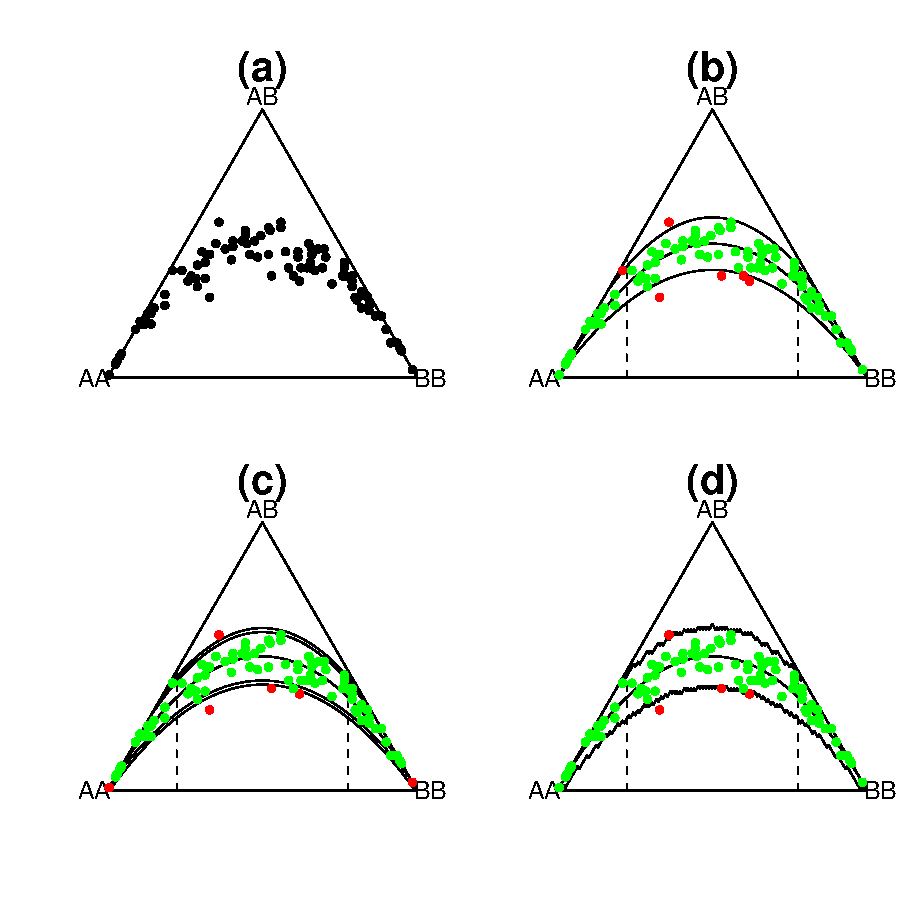
\includegraphics{HardyWeinberg-008}
\caption{Ternary plot of 100 simulated SNPs for 100 individuals. (a): ordinary ternary plot, (b): with $\chi^2$-acceptance
region, (c) with acceptance region for $\chi^2$-test with continuity correction, (d): with acceptance region for two-tailed
FE test.}
\end{figure}
More examples with human SNP data are given in Graffelman \& Morales~(2008).

\clearpage

\section{Online documentation}
\label{sec:online}

The online documentation for the most important routines of the package is
included below.

\HeaderA{HWChisq}{Chi square tests for Hardy Weinberg equilibrium}{HWChisq}
\keyword{htest}{HWChisq}
\begin{Description}\relax
\code{HWChisq} performs the chi-square test for Hardy Weinberg
equilibrium with or without continuity correction.
\end{Description}
\begin{Usage}
\begin{verbatim}
HWChisq(X, cc = 0, verbose = FALSE)
\end{verbatim}
\end{Usage}
\begin{Arguments}
\begin{ldescription}
\item[\code{X}] \code{X} a vector containg the genotypic counts (AA,AB,BB).
\item[\code{cc}] \code{cc} the continuity correction parameter (default \code{cc = 0}).
\item[\code{verbose}] \code{verbose} = 1 prints results, \code{verbose} = 0 is silent.
\end{ldescription}
\end{Arguments}
\begin{Value}
\code{HWChisq} returns a list with the components:
\begin{ldescription}
\item[\code{chisq }] value of the chi-square statistic. NA is returned if the marker is monomorphic.
\item[\code{pval }] p-value of the chi-square test for Hardy-Weinberg equilibrium.
\item[\code{D }] Half the deviation from Hardy-Weinberg equilibrium for the AB genotype.
\item[\code{p }] allele frequency of A.
\end{ldescription}
\end{Value}
\begin{Author}\relax
Jan Graffelman \email{jan.graffelman@upc.edu}
\end{Author}
\begin{SeeAlso}\relax
\code{\LinkA{HWLratio}{HWLratio}}
\end{SeeAlso}
\begin{Examples}
\begin{ExampleCode}
x <- c(298,489,213)
names(x) <- c("MM","MN","NN")
HW.test <- HWChisq(x,verbose=TRUE)
\end{ExampleCode}
\end{Examples}


\HeaderA{HWData}{Generating marker data in Hardy-Weinberg Equilibrium}{HWData}
\keyword{datagen}{HWData}
\begin{Description}\relax
HWData takes samples from the multinomial distribution given
Hardy-Weinberg allele frequencies.
\end{Description}
\begin{Usage}
\begin{verbatim}
HWData(n = 100, nm = 100, pfixed = NULL, exactequilibrium = FALSE, pdist
= "runif",...)
\end{verbatim}
\end{Usage}
\begin{Arguments}
\begin{ldescription}
\item[\code{n}] the sample size.
\item[\code{nm}] the number of markers (or samples).
\item[\code{pfixed}] take a fixed allele frequency with value \code{pfixed}.
\item[\code{exactequilibrium}] generate data in exact HWE or use the multinomial distribution
\item[\code{pdist}] take a random allele frequency from a uniform or beta
distribution.
\item[\code{...}] specific parameters for the uniform or beta
\end{ldescription}
\end{Arguments}
\begin{Value}
\begin{ldescription}
\item[\code{Xt}] the genotypic counts.
\item[\code{Xc}] the genotypic compositions.
\end{ldescription}
\end{Value}
\begin{Author}\relax
Jan Graffelman (jan.graffelman@upc.edu)
\end{Author}
\begin{SeeAlso}\relax
HWTernaryPlot
\end{SeeAlso}
\begin{Examples}
\begin{ExampleCode}
n <- 100
nm <- 100
out <- HWData(n,nm)
\end{ExampleCode}
\end{Examples}

\HeaderA{HWLratio}{Likelihood ratio test for Hardy Weinberg equilibrium}{HWLratio}
\keyword{htest}{HWLratio}
\begin{Description}\relax
\code{HWLratio} performs the Likelihood ratio test for Hardy Weinberg equilibrium.
\end{Description}
\begin{Usage}
\begin{verbatim}
HWLratio(X, verbose = FALSE)
\end{verbatim}
\end{Usage}
\begin{Arguments}
\begin{ldescription}
\item[\code{X}] \code{X} a vector containing the genotypic counts (AA,AB,BB).
\item[\code{verbose}] \code{verbose} = 1 prints results, \code{verbose} = 0 is silent.
\end{ldescription}
\end{Arguments}
\begin{Value}
\code{HWLratio} returns a list with the components:
\begin{ldescription}
\item[\code{Lambda }] the likelihood ratio
\item[\code{G2 }] -2*log(Lambda)
\item[\code{pval}] the p-value
\end{ldescription}
\end{Value}
\begin{Author}\relax
Jan Graffelman \email{jan.graffelman@upc.edu}
\end{Author}
\begin{References}\relax
Weir, B.S. (1996) Genetic data analysis II. Sinauer Associates, Massachusetts. See Chapter 3.
\end{References}
\begin{SeeAlso}\relax
\code{\LinkA{HWChisq}{HWChisq}}
\end{SeeAlso}
\begin{Examples}
\begin{ExampleCode}
x <- c(298,489,213)
names(x) <- c("MM","MN","NN")
HW.test <- HWLratio(x,verbose=TRUE)
\end{ExampleCode}
\end{Examples}


\HeaderA{HWTernaryPlot}{Ternary plot with the Hardy-Weinberg acceptance region}{HWTernaryPlot}
\keyword{aplot}{HWTernaryPlot}
\begin{Description}\relax
\code{HWTernaryPlot} is a routine that draws a ternary plot for three-way genotypic compositions (AA,AB,BB), and represents
the acceptance region for different tests for Hardy-Weinberg equilibrium (HWE) in the plot. This allows for graphical
testing of a large set of markers (e.g. SNPs) for HWE. The (non) significance of the test
for HWE can be inferred from the position of the marker in the ternary plot. Different statistical tests for HWE
can be done graphically with this routine: the ordinary chisquare test, the chisquare test with continuity
correction and the Fisher exact test.
\end{Description}
\begin{Usage}
\begin{verbatim}
HWTernaryPlot(X, n, addmarkers = TRUE, newframe = TRUE, hwcurve = TRUE, 
vbounds = TRUE, mafbounds = FALSE, mafvalue = 0.05, axis = 0, region = 1, 
vertexlab = colnames(X), alpha = 0.05, vertex.cex = 1, pch = 19, cc = 0.5, 
markercol = "black", markerbgcol = "black", cex = 0.75, axislab = "", 
verbose = FALSE, markerlab = NULL, mcex = 1, connect = FALSE, curvecols = 
rep("black",5), signifcolour = TRUE, ...)
\end{verbatim}
\end{Usage}
\begin{Arguments}
\begin{ldescription}
\item[\code{X}] a matrix of \code{n} genotypic compositions (\code{n} rows, rows summing 1, 3 columns, AA, AB and BB respectively).
\item[\code{n}] the samples size (for a complete composition with no missing data). 
\item[\code{addmarkers}] represent markers by dots in the triangle (\code{addmarkers=TRUE}) or not \\ 
(\code{addmarkers=FALSE}). 
\item[\code{newframe}] allows for plotting additional markers in an already existing ternary plot. Overplotting
is achieved by setting \code{newframe} to \code{FALSE}. Setting \code{newframe = TRUE} (default) will 
create a new ternary plot. 
\item[\code{hwcurve}] draw the HW parabola in the plot (\code{hwcurve=TRUE)} or not (\code{hwcurve=FALSE}). 
\item[\code{vbounds}] indicate the area corresponding to expected counts > 5 (\code{vbounds=TRUE}) or not 
(\code{vbounds=FALSE}).
\item[\code{mafbounds}] indicate the area corresponding to MAF < \code{mafvalue}. 
\item[\code{mafvalue}] a critical value for the minor allele frequency (MAF).
\item[\code{axis}] draw a vertex axis \\
0 = no axis is drawn \\
1 = draw the AA axis \\
2 = draw the AB axis \\
3 = draw the BB axis \\
\item[\code{region}] the type of acceptance region to be delimited in the triangle \\ 
0 = no acceptance region is drawn \\
1 = draw the acceptance region corresponding to a Chi-square test \\ 
2 = draw the acceptance region corresponding to a Chi-square test with continuity correction \\
3 = draw the acceptance region corresponding to a Chi-square test with continuity correction for D > 0 \\
4 = draw the acceptance region corresponding to a Chi-square test with continuity correction for D < 0 \\ 
5 = draw the acceptance regions for all preceding tests simultaneously \\ 
6 = draw the acceptance region corresponding to a Chi-square test with continuity correction with the upper
limit for D > 0 and the lower limit for D < 0 \\
7 = draw the acceptance region corresponding to a two-sided Fisher exact test \\

\item[\code{vertexlab}] labels for the three vertices of the triangle 
\item[\code{alpha}] significance level (0.05 by default) 
\item[\code{vertex.cex}] character expansion factor for the labels of the vertices of the triangle. 
\item[\code{pch}] the plotting character used to represent the markers. 
\item[\code{cc}] value for the continuity correction parameter (0.5 by default). 
\item[\code{markercol}] vector with colours for the marker points in the triangle. 
\item[\code{markerbgcol}] vector with background colours for the marker points in the triangle. 
\item[\code{cex}] expansion factor for the marker points in the triangle. 
\item[\code{axislab}] a label to be put under the horizontal axis. 
\item[\code{verbose}] print information on the numerically found cut-points between curves of the acceptance region and 
the edges of the triangle. 
\item[\code{markerlab}] labels for the markers in the triangle. 
\item[\code{mcex}] character expansion factor for the labels of the markers in the ternary plot. 
\item[\code{connect}] connect the represented markers by a line in the ternary plot. 
\item[\code{curvecols}] a vector with four colour specifications for the different curves that can be used
to delimit the HW acceptance region. E.g. \code{curvecols=c("red",
        "green","blue","black","purple")} will paint
the Hardy-Weinberg curve red, the limits of the acceptance region for an ordinary chi-square test
for HWE green, the limits of the acceptance region for a chi-square test with continuity correction
when D > 0 blue and the limits of the acceptance region for a chi-square test with continuity 
correction when D < 0 black, and the limits of the FE acceptance region purple. 
\item[\code{signifcolour}] colour the marker points automatically according to the result of a signifance test 
(green markers non-siginficant, red markers significant). 
\code{signifcolour} only takes effect if \code{region} is set to 1, 2 or 7.
\item[\code{...}] other arguments passed on to the plot function (e.g. \code{main} for a main title). 
\end{ldescription}
\end{Arguments}
\begin{Value}
\begin{ldescription}
\item[\code{minp }] minimum allele frequency above which testing for HWE is appropriate (expected counts exceeding 5).
\item[\code{maxp }] maximum allele frequency below which testing for HWE is appropriate.
\item[\code{inrange }] number of markers in the appropriate range.
\item[\code{percinrange }] percentage of markers in the appropriate.
\item[\code{nsignif }] number of significant markers (only if \code{region} equals 1,2 or 7.)
\end{ldescription}
\end{Value}
\begin{Author}\relax
Jan Graffelman \email{jan.graffelman@upc.edu}
\end{Author}
\begin{References}\relax
Graffelman, J. and Morales, J. (2008) Graphical tests for Hardy-Weinberg equilibrium 
based on the ternary plot. \emph{Human Heredity} 65(2):77-84.
\end{References}
\begin{SeeAlso}\relax
\code{\LinkA{HWChisq}{HWChisq}}
\end{SeeAlso}
\begin{Examples}
\begin{ExampleCode}

nm <- 100 # number of markers
n <- 100
Xc <- HWData(n,nm)$Xc

HWTernaryPlot(Xc,100,region=1,hwcurve=TRUE,vbounds=FALSE,vertex.cex=2)
\end{ExampleCode}
\end{Examples}


\section*{Acknowledgements}

This work was partially supported by the Spanish grant SEJ2006-13537 This document was generated by 
Sweave~(Leisch, 2002).

\section{References}

Graffelman, J. \& Morales-Camarena, J. (2008) Graphical tests for Hardy-Weinberg equilibrium
based on the ternary plot. {\it Human Heredity} {\bf 65}(2): 77-84.\\

Hedrick, P. W. (2005) {\it Genetics of Populations}. Third edition. Jones and Bartlett Publishers,
Sudbury, Massachusetts.\\

Leisch, F. (2002) Sweave: Dynamic generation of statistical reports using literate data analysis.
{\it Compstat 2002, Proceedings in Computational Statistics}. pp. 575-580, Physica Verlag, Heidelberg.
ISBN 3-7908-1517-9 URL http:/www.ci.tuwien.ac.at/~leisch/Sweave.\\

Weir, B. S. (1996) {\it Genetic Data Analysis II}. Sinauer Associates, Massachusetts.\\

\end{document}
